\chapter{Work and Energy}
\label{sec: work and energy}

\section{Forces and Work}
In principle using the contents of the previous sections, Newton's laws, momentum, and the kinematic equations, we can solve pretty much any problem in mechanics. However, Newton's laws are not always easy to apply. We say before that working with momentum gave us one way to study objects in motion without using Newton's laws directly. Another approach is to think in terms of \textbf{work} and \textbf{energy}.\\

Energy is another quantity that is conserved, though it can change form so the energy of a given type is not conserved as we will see when we study collisions later. We will concentrate on three types of energy:
\begin{itemize}
\setlength{\itemsep}{-5pt}
    \item \textbf{Work} -- the use/absorption of energy by movement.
    \item \textbf{Kinetic energy} -- Mechanical energy or energy of motion.
    \item \textbf{Potential energy} -- the energy that an object has due to its position.
\end{itemize} 

\paragraph{Work:} Work is done on an object when a force acts on it making it move, an object can also do work if energy is transferred away from an object through the application of a force. The work depends on the force and the distance the object moves, as well as the path the object moves along. The greater the force, or the distance moved, the greater the work done. By this we mean that Work = Force $\times$ distance. \\

The unit of work is the \textbf{Joule} (J) defined as the work done when a $1$N force moves an object a distance of $1$m. As an equation we have:
\begin{equation*}
W=Fs.
\end{equation*}
However, both force and displacement are vectors so what happens if they are not in the same direction? Then we are taking the vector product of $F$ and $s$ so a factor of $\cos\theta$, where $\theta$ is the angle between the two vectors appears,
\begin{equation*}
W=Fs\cos\theta.
\end{equation*}
To see this consider a yacht being acted on by the wind with a force $F$. There is an angle $\theta$ between the direction that the yacht moves in and the direction of the wind. This means that the force has a component $F\cos\theta$ in the direction of motion, and a component $F\sin\theta$ perpendicular to the motion. If the yacht moves a distance $s$ then the work done is $W=Fs\cos\theta$ as given above.  What do you think happens is $\theta=90^{\circ}$?

What we have said so far is only really true for a constant force. If the force depends on position or on time, then we need to be more careful. For a constant force, if we plot force against distance we see that the work done is the area under the curve, as they are both $Fs$.\\

The relationship between the work done and the area under a force distance plot still holds true even if the force is not constant, in fact what is actually going on is that the work done is the \textbf{integral} of the force along the path. As integration is beyond the scope of this module we mainly work with either constant forces, or forces with particularly simple position dependence.

\begin{figure}[ht]
    \centering
    \ThisAltText{ A mass on the end of a spring oscillating around equilibrium. }
    %\pdftooltip{
    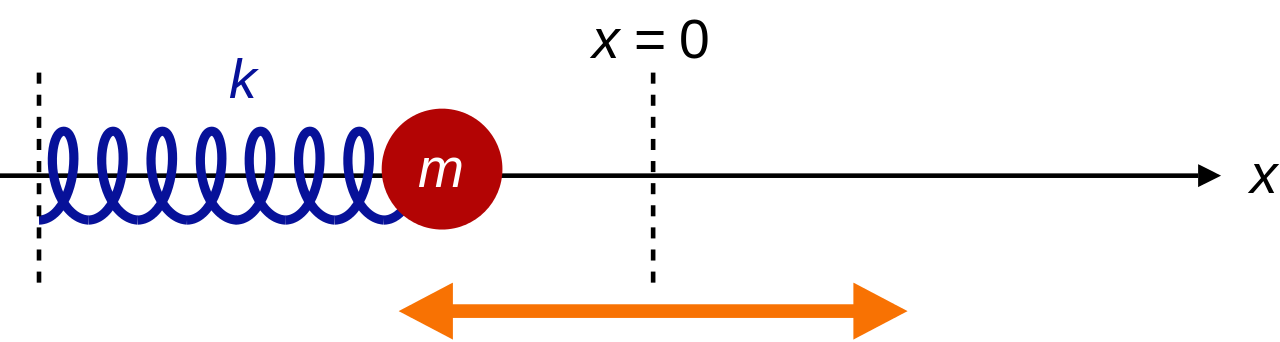
\includegraphics[width=0.6\textwidth]{figures/SHO_lagrangian_mech.png}
    %}{An oscillating spring}
    \caption{A spring with a mass on the end oscillating around equilibrium at $x=0$.}
\end{figure}

\paragraph{Example 5.1:} Consider the work done to stretch a spring. The greater the force, the more the spring stretches. The force needed to stretch the spring is proportional to its extension, $F= kx$, this is a version\footnote{For completeness note that here the force is a force acting on the spring to extend it, thus the force is pointing in the positive direction, when we return to Hooke's law in later weeks we will be discussing the springs natural restoring force which always points towards equilibrium, in that case the sign in Hooke's law will be negative.} of what is called \textbf{Hooke's Law}. We will return to Hooke's law in detail later in the module. The constant of proportionality $k$ that appears in Hooke's law is called the \textbf{spring constant} and it is a measure of how stiff, or difficult to stretch a spring is. If we plotted force against extension for Hooke's law we get a straight line, and the area under the line is the area of a triangle of base $x$ and height $F$. Thus
\begin{equation*}
W_{\text{spring}}=\frac{1}{2}F x=\frac{1}{2}k x^{2}.
\end{equation*}

\begin{figure}[ht]
    \centering
    \ThisAltText{ A plot of force against extension for a spring showing that there is a linear relationship.}
    %\pdftooltip{
    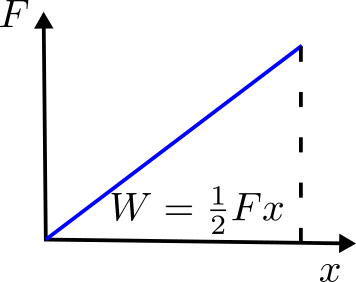
\includegraphics[width=0.4\textwidth]{figures/spring_work.png}
    %}{force against extension for a spring}
    \caption{A plot of applied force against extension for a spring.}
    \label{fig: spring extension}
\end{figure}


\paragraph{Kinetic Energy:} Kinetic energy is the energy of an object due to its motion. The faster an object moves the more kinetic energy it has. Kinetic energy is denoted by $K$ or $E_{K}$ and is also measured in Joules. We will make a lot of use of it when understanding how objects are moving. Note that for our purposes we can think of energy as a book keeping tool in the same way as momentum, though it plays quite a fundamental roll in understanding many areas of physics.\\

We can derive an equation for kinetic energy by making use Newton's second law, the formula for work, and one of the kinematic equations. Consider an object of mass $m$ starting at rest and acted on by a force $F$, resulting in it having a velocity $v$ after a time $t$. While accelerating the object has travelled
\begin{equation*}
s=\frac{1}{2}\left(u+v\right)t=\frac{1}{2}vt,
\end{equation*}
and has an acceleration of $a=\frac{v}{t}$. From Newton's second law we know that the force is given by
\begin{equation*}
F=ma=\frac{mv}{t}.
\end{equation*}
Thus the work done is
\begin{equation*}
W=Fs=\frac{1}{2}mv^{2}.
\end{equation*}
The object has gained energy from the work being done on it.

This expression holds true more generally and we call 
\begin{equation}
E_{K}=\frac{1}{2}mv^{2}
\label{eq: kinetic energy}
\end{equation}
the kinetic energy.

%
\paragraph{Potential Energy:}  Another type of energy that is relevant to the study of moving objects is the \textbf{potential energy}. This is the energy that an object has due to its position. Think of an object at rest at the top of a hill. It has no kinetic energy, but a lot of potential energy as it could gain potential energy by rolling down the hill. Sometime we would say that the object has the potential to do work.\\

If an object of mass $m$ is raised a vertical height $\Delta h$ as a steady speed, the force needed to raise the object is equal and opposite to its weight $W=mg$. Think of picking up an apple or a bag of sugar, you have to exert a force that balances teh weight of teh object to pick it up. The work done is then
\begin{equation*}
W=Fs=mg\Delta h.
\end{equation*}
The object now has the potential to do work if it falls so the (gravitational) potential energy is 
\begin{equation}
E_{P}=mg\Delta h.
\label{eq: potential energy}
\end{equation}

Note that some places will use $K$ for   kinetic energy and $U$ or $V$ for potential energy. In this module we will try to stick with $E_{K}$ and $E_{P}$ but be warned that not every book uses this notation.\\

\textbf{Warning:} Energy is a scalar quantity and as such is always positive\footnote{At least in most conventions, though you may find some older books that do not follow this approach.}, you may object to this saying that in $E_{P}$ we have $g$ and that is negative. However, when working with potential energy we are really working with $\vert g\vert =9.8\text{m/s}^{2}$. The formula is almost never quoted with the modulus signs and it is usually left to the reader to understand what is going on. Here, we will try to make clear the situations when we are really talking about $g$ and when we are talking about $\vert g\vert$.\\

Energy can change form between kinetic and potential, and other forms of energy that you may meet later on.  This was already suggested when we discussed how an object with potential energy at the top of a hill can lose potential energy, but gain kinetic energy by rolling down the hill. Consider an object of mass $m$ that has been raised to a height $h$, such that it has potential energy $E_{P}=mgh$. If the object is released it will accelerate as it falls, and the potential energy will become kinetic energy. After falling a distance $s$ it has kinetic energy equal to the change in kinetic energy
\begin{equation*}
\frac{1}{2}mv^{2}=mg h.
\end{equation*}
Note that since $g$ is only approximately constant \textbf{near} the surface of the Earth, if an object falls a great distance, or from a very great height, we will need to take account of the change in $g$.\\

Note that the conversion between kinetic and potential energy will not always be perfect, if there is air resistance, or friction of some kind then energy can be lost to heat or sound, and the gain in kinetic energy will be less than the loss of potential energy. We think of this loss as being due to an average frictional force acting over the whole of the objects motion. This force is found by associating the difference between the potential and kinetic energy with a work done by the object on the air or on the track that it is moving along. Then the average frictional force is given by
\begin{equation*}
F=\frac{W}{s}=\frac{E_{P}-E_{K}}{s}.
\end{equation*}

\paragraph{Example 5.2:} Consider a fairground ride whose track descends a vertical drop of $55\text{m}$ over a section of rails of length $120\text{m}$. A train of mass $2500\text{kg}$ on the track reaches a speed of $30\text{m/s}$ at the bottom of the descent after being at rest at the top. Find:
\begin{itemize}
\setlength{\itemsep}{-5pt}
    \item[a)] The potential energy lost by the train after descending.
    \item[b)] The gain in potential energy after the train has reached the bottom.
    \item[c)] The average frictional force on the train during the descent.
\end{itemize} 
a) The loss in potential energy is given by
\begin{equation*}
E_{P}=mg\Delta h=2500\times 9.8\times 55=1.35\times 10^{6}\text{J}.
\end{equation*}

b) The kinetic energy starts as $0\text{J}$ since the train is at rest, at the bottom it is
\begin{equation*}
E_{K}=\frac{1}{2}mv^{2}=\frac{1}{2}\times 2500\times (30)^{2}=1.13\times 10^{6}\text{J}.
\end{equation*}

c) The work done by the train on the rails and on the air is the difference between $E_{K}$ and $E_{P}$, $W=E_{P}-E_{K}=2.2\times 10^{5}\text{J}$, so the average frictional force is
\begin{equation*}
F=\frac{W}{s}=\frac{2.2\times 10^{5}}{120}=1830\text{N}.
\end{equation*}

\section{Power and Efficiency}
Energy can be transferred from one object to another in several ways. We have already seen that when an object rolls down a hill or falls down that the gravitational potential energy is transferred into kinetic energy. Energy is also transferred when an object does work, for example it causes a force to act on another object and transfers its energy to the other object, we will meet examples of this later when we discuss what happens to energy during a collision.\\

In the example that we saw earlier of potential energy swapping to kinetic energy imperfectly we said that the object lost energy to friction with the track and air resistance. This energy has not disappeared but has become heat energy or sound energy.  Since heat is a kind of energy\footnote{The study of heat is known a \textbf{thermodynamics} and is a major area of physics. Those of you on engineering and physics degrees will learn more about thermodynamics in future modules.}, the transfer of heat between objects is another kind of energy transfer. Heat can be transferred in essentially three ways: \textbf{Conduction}, \textbf{Convection}, \textbf{Radiation}. In addition, electricity, sound waves, and electromagnetic radiation\footnote{like light} will all transfer energy.\\

\textbf{Power} is the rate of transfer of energy, or the rate of change of energy. The unit of power is the Watt, with $1\text{W}=1 \text{J}/\text{s}$. The units is named after James Watt a Scottish inventor and engineer who was an early pioneer of steam engines. Mathematically the relationship between power, $P$, energy, $E$, and time, is given by
\begin{equation}
P=\frac{\Delta E}{\Delta t}.
\label{eq: PET equation}
\end{equation}
As was the case with the other rates of change we have met, this formula just gives the average power. The instantaneous power is given by the derivative of the energy. The formula is often given without the deltas as shown in the frmula triangle in \cref{fig: PEt triangle}. If a force does work then the power is the work done per second or 
\begin{equation*}
P=\frac{\Delta W}{\Delta t}.
\end{equation*}

\begin{figure}[ht]
    \centering
    \ThisAltText{ The formula triangle for energy, power, and time.}
    %\pdftooltip{
    \large \formulatriang[.4]{$E$}{}{$ P$}{}{$ t$}{}
    %}{The formula triangle for power, change in energy, and change in time.}
    \caption{The formula triangle for power, change in energy, and change in time. }
    \label{fig: PEt triangle}
\end{figure}

\paragraph{Example 5.3:} Consider a person of weight $690\text{N}$ who climbs a slight of stairs with height $10\text{m}$ in $12\text{s}$.  What is the power of their leg muscles?\\

The work done is:
\begin{align*}
W	&=Fs\\
	&=690\times 10=6900 \text{J}.
\end{align*}
The power due to this work done is then
\begin{align*}
P&=\frac{W}{t}\\
	&=\frac{6900}{12}\\
	&=575\text{W}.
\end{align*}
Thus each leg has a muscle power of $287.5\text{W}$.\\

For an engine the output power is sometimes called the \textbf{motive power}, as it is power available to cause motion, such as a steam engine on a train where the output power of the engine is used to move the train. For a powered vehicle driven by a constant force $F$ to move at a speed $v$, the power is given by
\begin{equation*}
P=Fv.
\end{equation*}
Can you see how to derive this from \cref{eq: PET equation} given the relationship between work done and force?

\paragraph{Example 5.4:} Consider an aircraft powered by engines which exert a force of $40\text{kN}$. The aircraft is in level flight at a constant velocity of $80\text{m/s}$. Calculate the power output of the engines at this speed.\\

First note that since we know a force and a velocity we will want to use $P=Fv$ to compute the power. We are given that $F=40\text{kN}=40000\text{N}$, and $v=80\text{m/s}$, thus
\begin{equation*}
P=Fv=40000\times 80 = 3.2\times 10^{6}\text{W}.
\end{equation*}


\paragraph{Example 5.5:} A person of weight $450\text{N}$ climbed $2.5\text{m}$ up a rope in $18\text{s}$. Calculate:
\begin{itemize}
\setlength{\itemsep}{-5pt}
    \item[a)] The gain in potential energy.
    \item[b)] The useful energy transfer per second, this is another name for the power.
\end{itemize} 

a) Use $E_{P}=mg\Delta h$ with $mg =450\text{N}$ and $\Delta h= 2.5$ so that
\begin{equation*}
E_{P}=mg\Delta h=450\times 2.5 =1125\text{J}\simeq 1.1\text{kJ}.
\end{equation*}

b) The useful energy transfer is the power and $P=W/t$ so 
\begin{equation*}
P=\frac{E_{P}}{t}=\frac{1125}{18}=62.5\text{W}.
\end{equation*}

\paragraph{Example 5.6:} An electric motor operating a sliding door exerts a force of $125\text{N}$ on the door causing it to open at a constant speed of $0.4 \text{m/s}$. What is the output power of the motor?\\

The output power is given by
\begin{equation*}
P=Fv=125\times 0.4 =50\text{W}.
\end{equation*}
The motor must transfer $50\text{J}$ of energy to the door every second while it is being opened.\\

Does all the energy supplied to the motor get used to open the doors? No, friction in the motor's bearings and electrical resistance in the wires mean that some of the electrical energy supplied to the motor is wasted. There will also be energy wasted if the motor makes a noise while it is working. For example, if the motor gets electrical energy at a rate of $150\text{J/s}$ and transfers $50\text{J/s}$ to the door then $100\text{J/s}$ is wasted due to friction, resistance, and sound. The fact that not all of the energy used is useful brings us on to the concept of \textbf{efficiency}.\\

The efficiency is the ratio of the useful energy to the total energy. It is often given the symbol $\epsilon$ and is given by the formula
\begin{equation*}
\epsilon =\frac{\text{Useful energy}}{\text{Total energy supplied}}.
\end{equation*}

\paragraph{Example 5.7:}  A $500\text{W}$ electric winch raises a $150\text{N}$ weight by $6\text{m}$ in $10\text{s}$. How much energy is wasted and what is the efficiency of the winch?\\

The electrical energy supplied to the winch while it is opperating is
\begin{equation*}
E=Pt=500\times 10=5000\text{J} = 5\text{kJ}.
\end{equation*}
However, the useful energy is the energy required to lift the weight, i.e. the potential energy gain of the weight which is
\begin{equation*}
\Delta E_{P}=mg \Delta h=150\times 6=900\text{J}=0.9\text{kJ}.
\end{equation*}
The diffrence between these two is the wasted energy
\begin{equation*}
\Delta E= E-\Delta E_{P}=5-0.9=4.1\text{kJ},
\end{equation*}
the efficiency is thus 
\begin{equation*}
\epsilon =\frac{0.9}{5}=0.18.
\end{equation*}

As well as expressing the efficiency using $\epsilon$, sometimes you will come across the percentage efficiency. This is just $\epsilon\times 100\%$. So in the last example the efficiency is $18\%$. We can also talk about efficiency whenever we have a change of energy, for example when we discussed the frictional force acting on moving objects we could also have phrased that as an efficiency. \\

A problem that people often study, particularly in material science of branches of engineering, is how to boost the efficiency when transferring energy. This is often rephrased as saying ``Is it possible to stop energy being lost as heat or sound?''\\

Consider a petrol or diesel engine in a car. This loses a lot of energy to heat as well as to sound. We could stop the engine loosing heat to the environment by insulating it, but then the engine would heat up itself until it stops working.  A similar example is a filament light bulb. These work by passing a current through a piece of wire, the filament, with a high resistance so that the wire will heat up and glow, creating light. In a sense the light is just a by product of the filament heating up. For example a filament bulb is around $12\%$ efficient with most of the energy wasted as heat, a fluorescent lamp is around $80\%$ efficient, and LED lights can be even better.\\

We can also think about the different sources of energy that we use to power our homes, in particular the renewable sources of energy like wind, solar, and hydro. In \textbf{STM0002 Group Project} the computer science and engineering students will see more about this and one of the project options is to explore different types of renewable energy generation. The important point here is that different types of energy generation will have different efficiencies, for example a wind turbine can be at most $60\%$ efficient, this is known as Betz's law and it can be fun to think about why there is this theoretical efficiency limit and what it means.\\

Since power is energy per second we can also think of the efficiency as the ratio of the usable power to the total power produced. This is particularly useful when thinking about power stations as the usable power will be the electrical power generated, while the total power is the energy supplied per second by the fuel, e.g. by burning coal or gas, or from the wind.

\paragraph{Example 5.8:} Consider a power station with an overall efficiency of $35\%$ which produces $200\text{MW}$ of electrical power. The fuel used in the power station releases $80\text{MJ}$ per kilogram of fuel burned. Calculate:
\begin{itemize}
\setlength{\itemsep}{-5pt}
    \item[a)] The energy per second supplied by the fuel,
    \item[b)] The mass of fuel that is burned per day.
\end{itemize} 

a) The energy per second supplied by the fuel is the total power, recall that $P=E/t$. We know that the power station is $35\%$ efficient so
\begin{equation*}
0.35=\frac{200\text{MW}}{\text{energy supplied per second}}
\end{equation*}
so
\begin{equation*}
\text{energy supplied per second}=\frac{200000}{0.35}=570\frac{\text{MJ}}{\text{s}}.
\end{equation*}

b) We get $80\text{MJ}$ for every kilogram of fuel burned so we need to burn $570/80=7.125\text{kg}$ every second to supply the claimed power. Thus we need to burn 
\begin{equation*}
7.125\times 60\times 60\times 24=6.2\times10^{5}\text{kg}
\end{equation*}
of fuel every day.


\section{Energy and Collisions}
In the last section we analysed collisions using conservation of momentum, at the end we said that there are two types of collision:
\begin{itemize}
\setlength{\itemsep}{-5pt}
    \item Elastic collisions where both momentum and kinetic energy are conserved.
    \item Inelastic collisions where momentum is conserved but the kinetic energy is not.
\end{itemize} 
Sometimes a distinction is made between inelastic collisions where the kinetic energy decreases, just called inelastic, and where the kinetic energy increases, called \textbf{explosions}. \\

In an inelastic collision either some of the kinetic energy is transferred into another kind of energy such as heat, or a different kind of energy, such as chemical energy, is transferred into kinetic energy. If we looked at the total energy rather than just the kinetic energy we would see that the total energy is conserved.\\

\paragraph{Example 5.9:} A ball of mass $m$ falls from a height $H$ and rebounds off the floor to a height $h$. How does the kinetic energy change during the motion?\\

The kinetic energy before the impact is the loss of potential energy when the ball falls from its original height, $E_{P}=mgH$. While the kinetic energy after the impact will be equal to the potential energy that the ball has when it reaches the new height $h$, $E_{P}=mgh$. If the kinetic energy is conserved (ie the collision is elastic) then $h=H$ and the ball returns to the height it started at. However, if the collision with the floor produces sound or the floor heats up the the final height will be less than the initial height, $h<H$ and the collision was inelastic.

\paragraph{Example 5.10:} Consider a railway wagon of mass $8000\text{kg}$ moving at $3.0\text{m/s}$ before colliding with an initially stationary wagon of mass $5000\text{kg}$. The two wagons separate after the collision, and the $8000\text{kg}$ wagon moves at a speed of $1\text{m/s}$ without changing its direction. Calculate:
\begin{itemize}
\setlength{\itemsep}{-5pt}
    \item[a)] The speed and direction of the $5000\text{kg}$ wagon after the collision,
    \item[b)] The change in kinetic energy of the wagons due to the collision.
\end{itemize} 

a) The initial momentum is 
\begin{equation*}
p_{i}=8000\times 3 +5000\times 0=24 000\frac{\text{kg m}}{\text{s}}.
\end{equation*}
Let us call the final velocity of the $5000\text{kg}$ wagon $v_{B}$, then the final momentum is
\begin{equation*}
p_{f}=8000\times 1 +5000\times v_{B}=8000+5000v_{B}.
\end{equation*}
Conservation of momentum implies that $p_{i}=p_{f}$ or that
\begin{align*}
24 000&=8000+5000v_{B},\\
\Rightarrow v_{B}&=\frac{24000-8000}{5000}\\
&=\frac{16000}{5000}=3.2\text{m/s}.
\end{align*}
So the $5000\text{kg}$ wagon is moving in the same direction as the $8000\text{kg}$ wagon but at a speed of $3.2\text{m/s}$.\\

b) Now we repeat the same analysis but calculate the kinetic energies rather than the momentum. The inital kinetic energy is
\begin{equation*}
E_{K_{i}}=\frac{1}{2}\times 8000\times(3)^2 +\frac{1}{2}\times 5000\times 0=36000\text{J}.
\end{equation*}

After the collision the kinetic energy is
\begin{equation*}
E_{K_{f}}=\frac{1}{2}\times 8000\times 1^{2}+\frac{1}{2}\times 5000\times (3.2)^{2}=29 600\text{J}.
\end{equation*}

The change in kinetic energy is then
\begin{equation*}
E_{K_{i}}-E_{K_{f}}=36000-29600=6400\text{J}.
\end{equation*}
Thus the total kinetic energy of the system has decreased by $6400\text{J}$.\\


Several of the problems on the tutorial sheet will get you to revisit collisions that you have previously studied using momentum so that you can see what happens to the mechanical energy in these cases.